\documentclass[journal]{IEEEtran}

\usepackage{amsmath,amssymb}
\usepackage{booktabs}
\usepackage{graphicx}
\usepackage{url}
\usepackage[hidelinks]{hyperref}
\usepackage{cite}

\graphicspath{{figures/}}

\begin{document}

\title{SkillEvo: Calibrated Skill Selection and Tiered Experience Memory for Cross-Task Transfer in Spatiotemporal Agents}

\author{Jiabei Zheng%
\thanks{Manuscript prepared for the IEEE Journal of Selected Topics in Applied Earth Observations and Remote Sensing (JSTARS).}}

\maketitle

\begin{abstract}
Spatiotemporal agents increasingly rely on libraries of reusable analysis procedures (skills) induced from earlier remote-sensing workflows. The central question is not only how to retrieve a skill, but whether a retrieved skill will actually be reusable on a new task. Description embeddings answer the first question and are frequently used as a proxy for the second. We show that this proxy is brittle: lexically similar recipes can encode incompatible spectral mechanisms, input cardinality, or target semantics. We present SkillEvo, a module that combines a small calibrated reuse discriminator, a two-tier experience memory, and a transferability diagnosis for cross-task skill gating. The discriminator predicts the probability that a historical skill will succeed on a new task from retrieval and structural compatibility, with an optional family-conditioned memory variant; isotonic regression calibrates its probabilities on held-out tasks. The memory keeps recent episodes verbatim and consolidates long-term experience through deduplication and bounded compression. The transfer diagnosis estimates a Beta-binomial posterior over positive transfer on a small target probe split and blocks skills with weak structural and empirical support. On a controlled seven-family spatiotemporal benchmark, the calibrated selector raises top-1 success from 0.500 (description embedding) to 0.675 and mean task score from 0.505 to 0.629, while improving AUROC from 0.666 to 0.842 and reducing expected calibration error from 0.152 to 0.063. Transfer gating raises success to 0.698 and reduces negative transfer from 0.056 to 0.048. Tiered memory preserves success while reducing the retained experience footprint by 5.7$\times$ relative to flat memory and substantially improving calibration over a no-memory agent. A feature ablation shows that structural compatibility carries most of the selection signal in this benchmark; historical statistics mainly improve calibration and enable bounded memory. The benchmark and code are released for reproduction.
\end{abstract}

\begin{IEEEkeywords}
skill selection, experience memory, calibration, transfer diagnosis, spatiotemporal agents, remote sensing workflows.
\end{IEEEkeywords}

\section{Introduction}

Remote-sensing analysis is increasingly assembled from reusable procedures: compute an index, threshold it, remove small components, fit a classifier on reference pixels, or compare two dates. Agents that solve such tasks can accumulate these procedures as a \emph{skill library} and reuse them on later tasks \cite{voyager,expel,awm}. Reuse is attractive because it saves exploration and encodes expert parameter choices. It is also risky: a water extractor applied to a change-detection task may produce a plausible map with the wrong semantics, and a single-date classifier cannot exploit bi-temporal evidence. The resulting \emph{negative transfer} is often invisible to retrieval scores.

Most agent memory and skill-selection systems rank candidates by embedding similarity to a task description \cite{rag,voyager,memorybank}. This is a reasonable recall mechanism but a weak decision rule. Embeddings conflate surface vocabulary with mechanism: ``water extraction from NDWI'' and ``flood mapping from NDWI'' are nearly identical in text, while ``change detection with spectral distance'' and ``land-cover classification'' may share many words yet require different inputs and outputs. Retrieval also ignores historical outcomes: a skill that repeatedly failed on a family should be down-ranked even if its description matches.

This paper asks three questions. (1) Can a small, calibrated discriminator predict skill reusability better than description similarity, and can its probabilities be trusted? (2) Can a two-tier memory retain the benefits of experience while keeping storage bounded and calibration stable? (3) Can a transferability score estimated from a few target probes isolate non-transferable skills and reduce negative transfer?

We answer them with \emph{SkillEvo}, outlined in Fig.~\ref{fig:architecture}. A semantic retriever proposes candidates from a deduplicated skill library. A calibrated logistic discriminator reranks them using retrieval and structural compatibility; a memory-enabled variant adds family-conditioned outcome statistics. A tiered memory supplies short-term and long-term evidence and is updated after each outcome. A transfer diagnosis runs each candidate on a small target development split, combines probe utility with a structural prior in a Beta-binomial score, and gates blocked skills before reranking.

\begin{figure}[t]
\centering
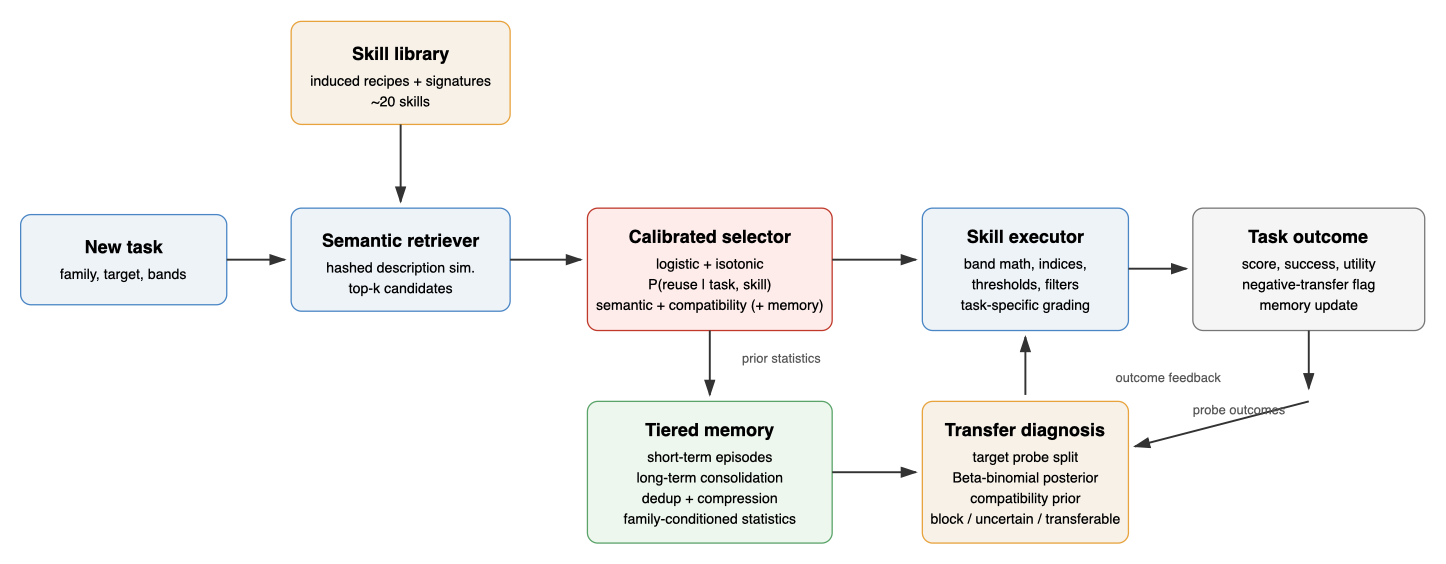
\includegraphics[width=\columnwidth]{architecture.png}
\caption{SkillEvo components. The selector combines retrieval, structural compatibility, and tiered memory. Transfer diagnosis uses a small target probe split to gate non-transferable skills.}
\label{fig:architecture}
\end{figure}

The contributions are:
\begin{itemize}
\item A calibrated skill-reuse discriminator that predicts $P(\text{reuse}\mid\text{task},\text{skill})$ and is calibrated post hoc with temperature scaling or isotonic regression. It improves top-1 success by 17.5 percentage points over description retrieval (McNemar $p<0.001$) and reduces ECE from 0.152 to 0.063.
\item A tiered experience memory with short-term verbatim episodes and long-term deduplicated/compressed records. It preserves success while shrinking retained experience by 5.7$\times$ relative to flat memory and reduces ECE from 0.232 to about 0.12 in a prequential stream.
\item A cross-task transfer diagnosis that blocks non-transferable skills, raises success from 0.675 to 0.698, and lowers negative transfer from 0.056 to 0.048. Its transferability matrix exposes interpretable block structure.
\item A controlled diagnostic benchmark and full reproduction package: seven spatiotemporal families, deterministic scenes, induced skill libraries, calibrated metrics, bootstrap intervals, paired tests, and a dependency-free implementation.
\end{itemize}

We are explicit about scope. The benchmark is synthetic and small. It is designed to isolate selection and transfer effects, not to establish state-of-the-art land-cover or change-detection accuracy. The feature ablation shows that structural compatibility alone is competitive with the full selector; we report this because it changes how the method should be used.

\section{Related Work}

\textbf{Skill libraries and agent memory.} Voyager \cite{voyager} stores executable code skills and retrieves them by description; ExpeL \cite{expel} extracts insights from success and failure trajectories; Reflexion \cite{reflexion} keeps verbal reflections; Agent Workflow Memory \cite{awm} induces reusable workflows. MemoryBank \cite{memorybank} and MemGPT \cite{memgpt} add long-term memory with summarization and paging. Generative Agents \cite{park} use a memory stream with recency, importance, and relevance. These systems establish that reuse and memory help, but they evaluate end-to-end with an LLM and rarely calibrate the reuse decision or diagnose cross-family transfer.

\textbf{Retrieval and reranking.} Dense retrieval \cite{dpr,rag} and late interaction \cite{colbert} rank passages by representation similarity. Skill selection is a retrieval problem with an important difference: the ranked item is executable, and its usefulness depends on input requirements and output semantics that a description may omit. Our discriminator is a lightweight reranker trained on observed skill outcomes rather than query-document relevance.

\textbf{Calibration.} Modern classifiers are often overconfident \cite{guo}. Temperature scaling, Platt scaling, isotonic regression, and beta calibration are standard post-hoc fixes \cite{platt,zadrozny,niculescu,kull}. We use temperature and isotonic calibration because they are cheap and interpretable. Calibration matters here because the score is used as a probability of reuse and because downstream gating and memory updates depend on it.

\textbf{Transfer and negative transfer.} Transfer learning studies when source knowledge helps a target task \cite{pan,zhuang}. Negative transfer is usually diagnosed after training. Our setting is episodic: a small number of target probes is available before the agent commits, so we estimate transferability online with a Beta-binomial posterior rather than retraining a model.

\textbf{Spatiotemporal and remote-sensing agents.} Deep learning has become standard for land-cover mapping and change detection \cite{zhu,ma,chencd}. Foundation models such as SpectralGPT \cite{spectralgpt}, RemoteCLIP \cite{remoteclip}, and SkySense \cite{skysense} provide general representations. Our benchmark deliberately avoids heavy representations: tasks are solved by explicit spectral and spatial operations so that skill reuse, not representation quality, is the experimental variable.

\section{Problem Formulation}

Let $\mathcal{L}=\{s_1,\dots,s_n\}$ be a skill library. A skill $s$ is a macro $(o_1,\dots,o_m)$ of primitive operations with a canonical signature, an input kind (single-date or bi-temporal), required bands, target labels, and provenance. A task $t$ has a family, a target, an input kind, band metadata, and a hidden ground-truth map. Executing $s$ on $t$ yields a prediction and a task metric $q(s,t)\in[0,1]$ (overall accuracy for multiclass maps, F1 for binary maps).

A task is \emph{solved} if $q(s,t)\ge\tau_f$, where $\tau_f$ is a family-specific acceptance threshold fixed before evaluation. The reuse label is
\begin{equation}
y(s,t)=\mathbf{1}\left[q(s,t)\ge\tau_f\right].
\end{equation}
Given a candidate set $C(t)$ returned by a retriever, the selector estimates $p(s,t)=P(y=1\mid t,s,M)$, where $M$ is the current memory. The agent executes the highest-scoring candidate (or retries up to a budget $B$). We evaluate both top-1 and budgeted selection.

The central comparison is between ranking by $p(s,t)$ and ranking by description similarity $\mathrm{sim}(\phi(t),\psi(s))$, where $\phi$ and $\psi$ are hashed text embeddings. Both use the same candidate pool, so the comparison isolates the reranker.

\section{Method}

\subsection{Skill Induction and Library}

Source tasks are solved by reference recipes. A recipe is a sequence of primitives such as \texttt{index(ndwi)}, \texttt{threshold(otsu)}, \texttt{spectral\_change}, \texttt{classify(nearest\_centroid)}, \texttt{smooth(majority)}, \texttt{remove\_small}, and \texttt{fill\_holes}. The reference recipe and its parameter variants are canonicalized; identical signatures are merged. A typical run yields about 20 skills. The library also stores provenance (source family and tasks), input requirements, targets, and a natural-language description used only for retrieval.

The generic fallback is a fixed NDVI threshold without cleanup. It is intentionally weak, so improvements measure the value of historical skills rather than the strength of a hand-coded baseline.

\subsection{Calibrated Reuse Discriminator}

The discriminator is an $L_2$-regularised logistic model fitted by iteratively reweighted least squares with class-balanced weights. Features fall into three groups.

\textbf{Retrieval.} Cosine similarity between hashed description embeddings and its rank among candidates.

\textbf{Compatibility.} Target match, source-family match, input-kind match, spectral-mechanism match (e.g., NDWI for water, spectral distance for change, nearest centroid for land cover), band coverage, adaptivity, and operation cost.

\textbf{Experience (optional memory variant).} Beta-smoothed success rate, mean utility, utility standard deviation, evidence strength, recency, family coverage, duplicate rate, novelty, recent success, and family-conditioned success from memory. The default selector uses the structural set; the memory variant is used for the streaming experiment.

The model outputs a logit; a post-hoc calibrator maps it to a probability. Temperature scaling learns one scalar $T$ by minimizing negative log-likelihood on a held-out source split:
\begin{equation}
p_T=\sigma\!\left(\frac{\mathrm{logit}}{T}\right).
\end{equation}
Isotonic regression fits a monotone step function by pool-adjacent-violators. We report both; the main model uses isotonic calibration. A variant calibrated on target development tasks measures few-shot adaptation.

\subsection{Tiered Experience Memory}

Memory receives an outcome record after each execution: skill, task family, target, success, utility, and a timestamp. The short-term tier keeps the last $W=24$ records verbatim. The long-term tier applies one of four policies: \texttt{tiered} (bounded FIFO truncation), \texttt{tiered\_dedup} (collapse records with the same skill, family, target, success, and utility bucket), and \texttt{full} (dedup plus utility-aware pruning during consolidation).

Statistics are computed from the long-term store, with the short-term store supplying recency and recent-success features. The design separates episodic evidence (recent, high-resolution) from semantic evidence (consolidated, bounded), following the distinction between fast and slow memory in agent architectures \cite{memgpt,park}.

\subsection{Cross-Task Transfer Diagnosis}

For a candidate skill and target family, the agent runs the skill on a small probe split of target development tasks. Let $u_i$ be the utility delta on probe $i$ (task score minus the generic baseline), $n$ the number of probes, and $k$ the number of positive deltas. A Beta posterior is
\begin{equation}
\alpha=1+2c+k,\qquad \beta=1+2(1-c)+(n-k),
\end{equation}
where $c$ is a structural compatibility score:
\begin{equation}
\begin{aligned}
c={}&0.30\,\mathrm{target}+0.15\,\mathrm{family}+0.15\,\mathrm{input}\\
&+0.30\,\mathrm{mechanism}+0.10\,\mathrm{band}.
\end{aligned}
\end{equation}
The transferability score combines compatibility and normalized probe utility:
\begin{equation}
r=0.60c+0.40\,\mathrm{clip}\!\left(\frac{\bar u+0.10}{0.60},0,1\right).
\end{equation}
A skill is \emph{blocked} if $c<0.35$ and $\bar u<0.25$; \emph{transferable} if strong probe evidence ($\bar u\ge0.25$, positive rate $\ge0.75$) overrides a weak prior, or if structural compatibility and positive utility agree, or if partial compatibility ($c\ge0.35$) meets positive utility ($\bar u>0.10$); otherwise it is \emph{uncertain}. Blocked skills are removed before reranking; uncertain skills are down-weighted. The thresholds are fixed on development data and not tuned on the test split.

\section{Benchmark and Protocol}

\subsection{Scenes and Tasks}

Each scene is $32\times32$ pixels with six bands (blue, green, red, NIR, SWIR1, SWIR2). Class-specific spectra are combined with spatially contiguous land cover, agricultural fields, seasonal illumination, sensor gain, texture, noise, and optional cloud contamination. Bi-temporal scenes apply controlled changes: urban expansion, deforestation, crop rotation, flooding, or fire. Task families are summarized in Table~\ref{tab:families}.

\begin{table}[t]
\centering
\caption{Task Families}
\label{tab:families}
\begin{tabular}{lllc}
\toprule
Family & Input & Target & Threshold \\
\midrule
Land cover & single & six classes (OA) & 0.78 \\
Crop & single & crop / non-crop (F1) & 0.55 \\
Water & single & water (F1) & 0.65 \\
Flood & single & post-event water (F1) & 0.60 \\
Change & two dates & any change (F1) & 0.40 \\
Urban & two dates & new urban (F1) & 0.45 \\
Burn & two dates & burn scar (F1) & 0.50 \\
\bottomrule
\end{tabular}
\end{table}

\subsection{Splits and Metrics}

We use three seeds. Per seed, 70 source training tasks (10 per family), 28 source validation tasks, 56 target development tasks (8 per family), 42 target test tasks (6 per family), and 56 stream tasks. Source and target tasks use disjoint scene seeds and parameter combinations.

The candidate pool is the top eight skills by description embedding. Main results use top-1 selection; a budgeted variant retries up to three candidates. We report success, mean task score, negative-transfer rate, AUROC, AUPRC, Brier score, NLL, ECE, precision at one, and NDCG at five. Confidence intervals use 2,000 task-level bootstrap resamples. Paired success uses an exact McNemar test; paired scores use a 5,000-draw sign-flip permutation test.

Negative transfer is counted when the selected skill falls back because it is incompatible, or when its utility is below $-0.02$. This is deliberately strict: a skill that is merely weaker than the best candidate but still improves on the generic baseline is not labeled harmful.

\section{Results}

\subsection{Skill Selection and Calibration}

Table~\ref{tab:main} reports the main comparison. Description retrieval solves 0.500 of target tasks. The calibrated selector solves 0.675, an improvement of 17.5 percentage points (McNemar $p<0.001$), and raises mean score from 0.505 to 0.629 (permutation $p=0.0002$). Ranking quality increases from AUROC 0.666 to 0.842 and AUPRC from 0.547 to 0.661. Brier score falls from 0.233 to 0.156.

\begin{table*}[t]
\centering
\caption{Main Results (Three Seeds, 126 Target Tasks)}
\label{tab:main}
\small
\begin{tabular}{lccccccccc}
\toprule
Method & Success & Score & Neg. transfer & AUROC & AUPRC & Brier & NLL & ECE & P@1 \\
\midrule
Random & 0.349 & 0.389 & 0.294 & 0.495 & 0.369 & 0.334 & 1.007 & 0.284 & 0.333 \\
Embedding & 0.500 & 0.505 & 0.183 & 0.666 & 0.547 & 0.233 & 1.127 & 0.152 & 0.500 \\
Frequency & 0.540 & 0.524 & 0.198 & 0.509 & 0.380 & 0.246 & 0.686 & 0.138 & 0.540 \\
Logistic & 0.683 & 0.632 & 0.056 & 0.842 & 0.655 & 0.164 & 0.491 & 0.120 & 0.683 \\
+ temperature & 0.683 & 0.632 & 0.056 & 0.842 & 0.655 & 0.165 & 0.494 & 0.105 & 0.683 \\
+ isotonic & 0.675 & 0.629 & 0.056 & 0.842 & 0.661 & 0.156 & 0.629 & 0.063 & 0.675 \\
+ target-dev cal. & 0.683 & 0.632 & 0.056 & 0.841 & 0.654 & 0.157 & 0.612 & 0.087 & 0.683 \\
Budgeted retry & 0.746 & 0.701 & 0.286 & 0.842 & 0.661 & 0.156 & 0.629 & 0.063 & 0.675 \\
Oracle bound & 0.802 & 0.753 & 0.000 & -- & -- & -- & -- & -- & -- \\
\bottomrule
\end{tabular}
\end{table*}

\begin{figure}[t]
\centering
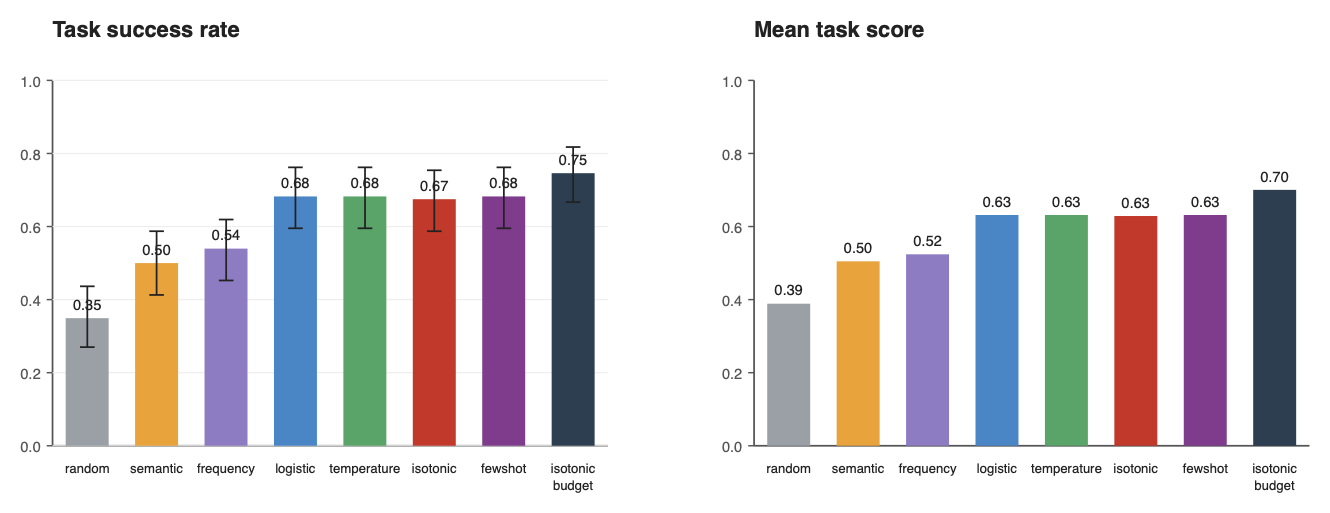
\includegraphics[width=\columnwidth]{methods.png}
\caption{Top-1 success with 95\% bootstrap intervals (left) and mean task score (right).}
\label{fig:methods}
\end{figure}

The uncalibrated logistic model is already discriminative (AUROC 0.842) but overconfident (ECE 0.120). Temperature scaling modestly improves ECE to 0.105; isotonic calibration cuts it to 0.063 and Brier to 0.156, at a small cost in top-1 success (0.675 vs 0.683). Target-development calibration reaches ECE 0.087, suggesting that a handful of labelled target tasks can substitute for source validation data. The budgeted retry closes most of the gap to the oracle bound (0.746 vs 0.802), at the cost of more attempts and a higher negative-transfer rate.

\begin{figure}[t]
\centering
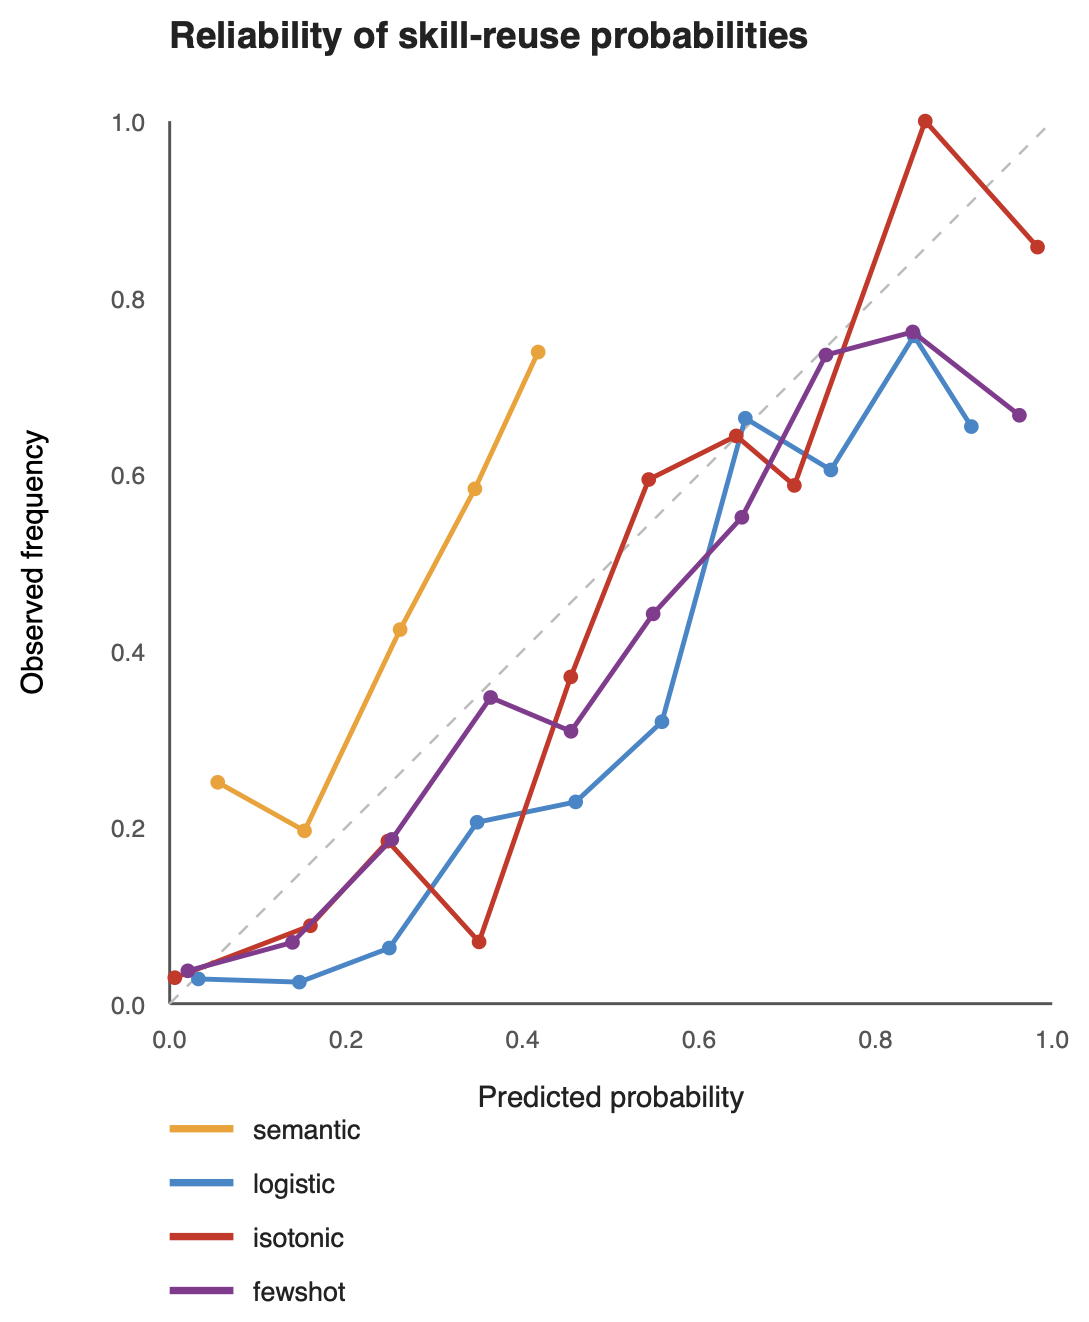
\includegraphics[width=\columnwidth]{reliability.png}
\caption{Reliability of reuse probabilities. The diagonal is perfect calibration.}
\label{fig:reliability}
\end{figure}

\subsection{Feature Ablation}

Table~\ref{tab:ablation} isolates feature groups. The structural set is the default discriminator and reaches 0.675 top-1 success. Adding historical outcome features lowers static top-1 success to 0.611; history-only features reach 0.579. The structural set also has the best ECE (0.063).

\begin{table}[t]
\centering
\caption{Feature Ablation (Isotonic Calibration)}
\label{tab:ablation}
\begin{tabular}{lcccc}
\toprule
Feature set & Success & Score & AUROC & ECE \\
\midrule
Semantic only & 0.500 & 0.504 & 0.664 & 0.073 \\
Structural & 0.675 & 0.629 & 0.842 & 0.063 \\
History & 0.579 & 0.586 & 0.784 & 0.073 \\
Curated & 0.619 & 0.613 & 0.852 & 0.070 \\
Full & 0.611 & 0.610 & 0.854 & 0.077 \\
\bottomrule
\end{tabular}
\end{table}

This is the most important negative result in the paper. On this benchmark, the structural features do most of the work; historical outcome statistics are noisy because the source corpus is small and contains many failed trials. History features still improve calibration in the streaming setting, where they are updated online, but they do not improve static top-1 selection. We therefore use the structural set for the default selector and treat history as a calibration and memory mechanism, not as a substitute for structural validation.

\begin{figure}[t]
\centering
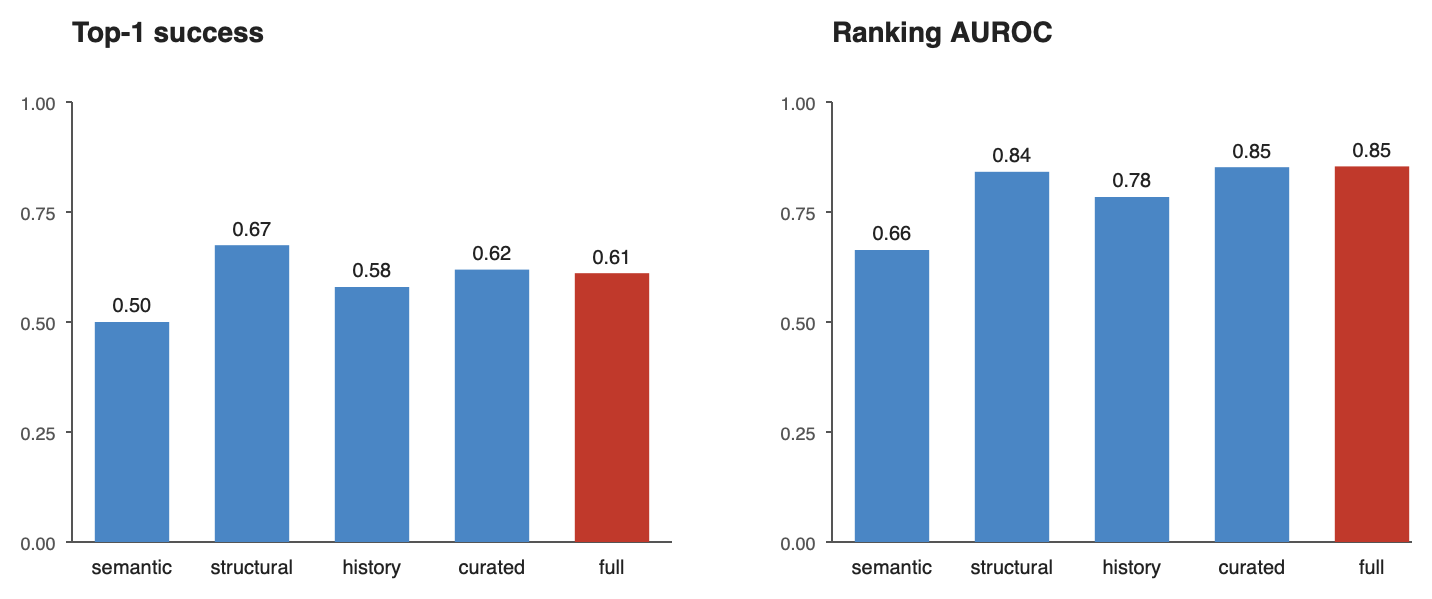
\includegraphics[width=\columnwidth]{ablation.png}
\caption{Feature ablation for top-1 success and ranking AUROC.}
\label{fig:ablation}
\end{figure}

\subsection{Cross-Task Transfer Diagnosis}

Table~\ref{tab:gate} reports gate strategies. The proposed gate raises success from 0.675 to 0.698 and lowers negative transfer from 0.056 to 0.048. A semantic compatibility gate is too aggressive (0.579): it blocks cross-family skills that empirical probes would have retained. Outcome-only gating does not help: probe utility alone is not sufficient because a weak skill can improve on a very weak baseline.

\begin{table}[t]
\centering
\caption{Transfer Gating (Top-1)}
\label{tab:gate}
\begin{tabular}{lccc}
\toprule
Strategy & Success & Score & Negative transfer \\
\midrule
No gate & 0.675 & 0.629 & 0.056 \\
Semantic gate & 0.579 & 0.559 & 0.103 \\
Outcome gate & 0.675 & 0.629 & 0.056 \\
Proposed & 0.698 & 0.647 & 0.048 \\
\bottomrule
\end{tabular}
\end{table}

\begin{figure}[t]
\centering
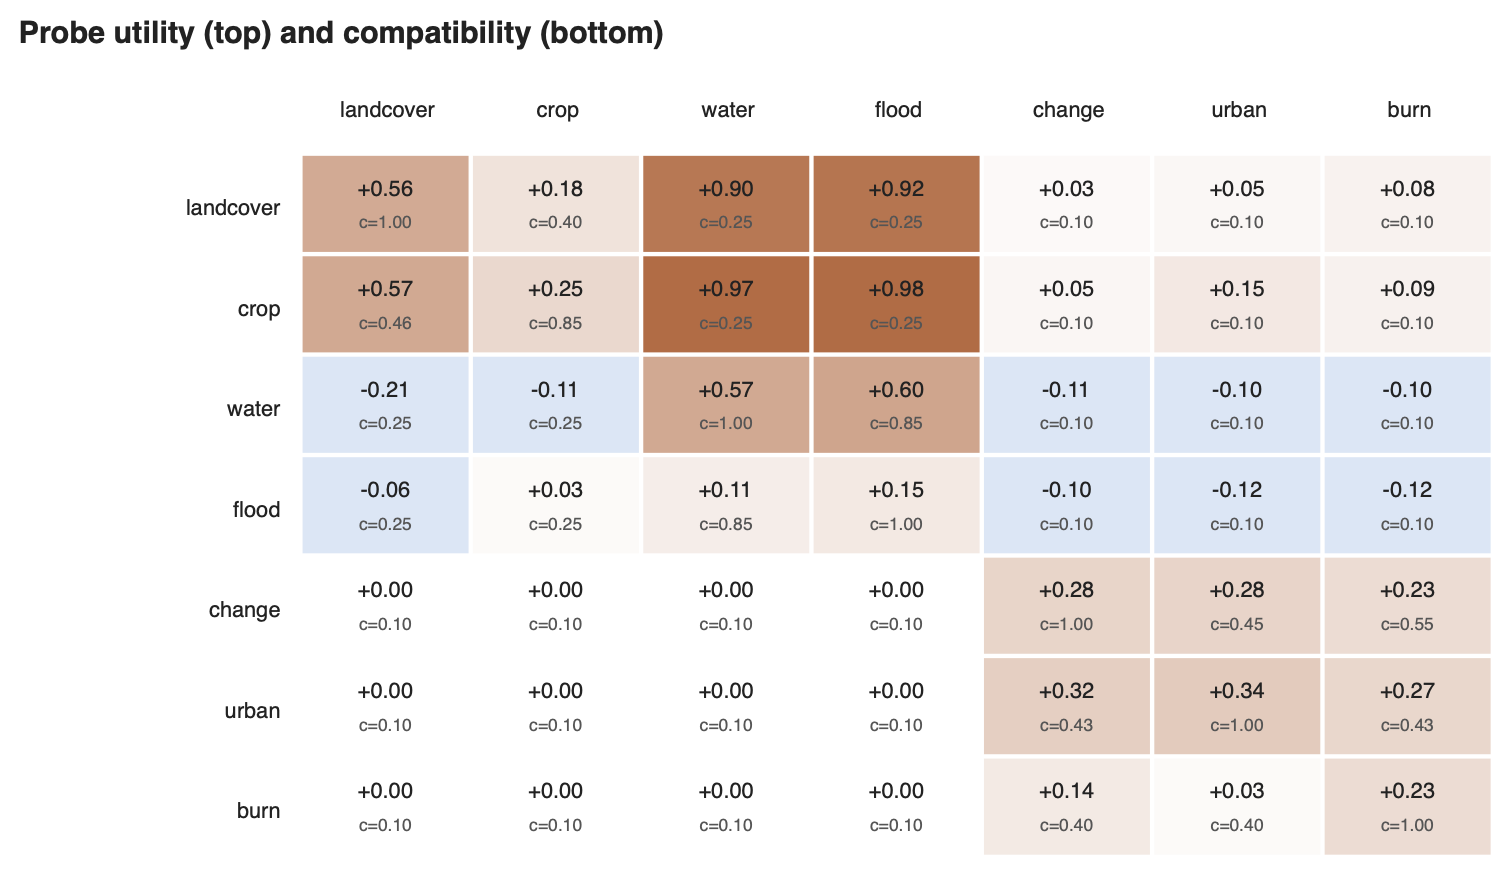
\includegraphics[width=\columnwidth]{transfer_heatmap.png}
\caption{Source-to-target probe utility (top) and structural compatibility (bottom).}
\label{fig:heatmap}
\end{figure}

The transferability matrix (Fig.~\ref{fig:heatmap}) exposes a block structure. Land-cover and crop classifiers transfer strongly to water and flood (probe utility 0.90--0.98) because the task supplies binary reference pixels and the classifier adapts. They do not transfer to change, urban, or burn (0.03--0.15). Water skills transfer to flood (0.60) but not to change ($-0.11$). Change and burn detectors transfer to each other (0.28/0.23). These patterns are consistent with the underlying mechanisms: single-date spectral classifiers and bi-temporal change detectors are different input regimes.

Pair-level case studies clarify the trade-off. On land-cover $\rightarrow$ change, all source skills are blocked; the un-gated agent occasionally succeeds by luck (0.06) but incurs frequent negative transfer, while the gated agent falls back to the generic baseline and succeeds on 0.00. The gate is doing what it claims---isolating non-transferable skills---but it cannot create a transferable skill that is not in the library. On water $\rightarrow$ flood, all skills are retained and success is 1.00. On land-cover $\rightarrow$ crop, partial compatibility keeps the classifiers and success is 0.61. On crop $\rightarrow$ land cover, success is 0.94.

\subsection{Tiered Memory}

Table~\ref{tab:memory} reports the prequential stream. Success is essentially flat across memory modes (0.774--0.786), but calibration improves sharply. No memory gives ECE 0.232; flat memory gives 0.113; tiered gives 0.131; full gives 0.120. The flat store keeps 616 records / 57,315 characters; the full store keeps 109 records / 9,987 characters, a 5.7$\times$ reduction. Deduplication keeps 104 records / 9,428 characters.

\begin{table}[t]
\centering
\caption{Prequential Memory Stream}
\label{tab:memory}
\small
\begin{tabular}{lcccccc}
\toprule
Mode & Success & Score & ECE & Records & Chars & Dup. \\
\midrule
None & 0.774 & 0.709 & 0.232 & 0 & 0 & 0.000 \\
Flat & 0.780 & 0.699 & 0.113 & 616 & 57,315 & 0.000 \\
Tiered & 0.780 & 0.703 & 0.131 & 106 & 9,535 & 0.000 \\
Tiered+dedup & 0.786 & 0.707 & 0.141 & 104 & 9,428 & 0.500 \\
Full & 0.774 & 0.705 & 0.120 & 109 & 9,987 & 0.492 \\
\bottomrule
\end{tabular}
\end{table}

\begin{figure}[t]
\centering
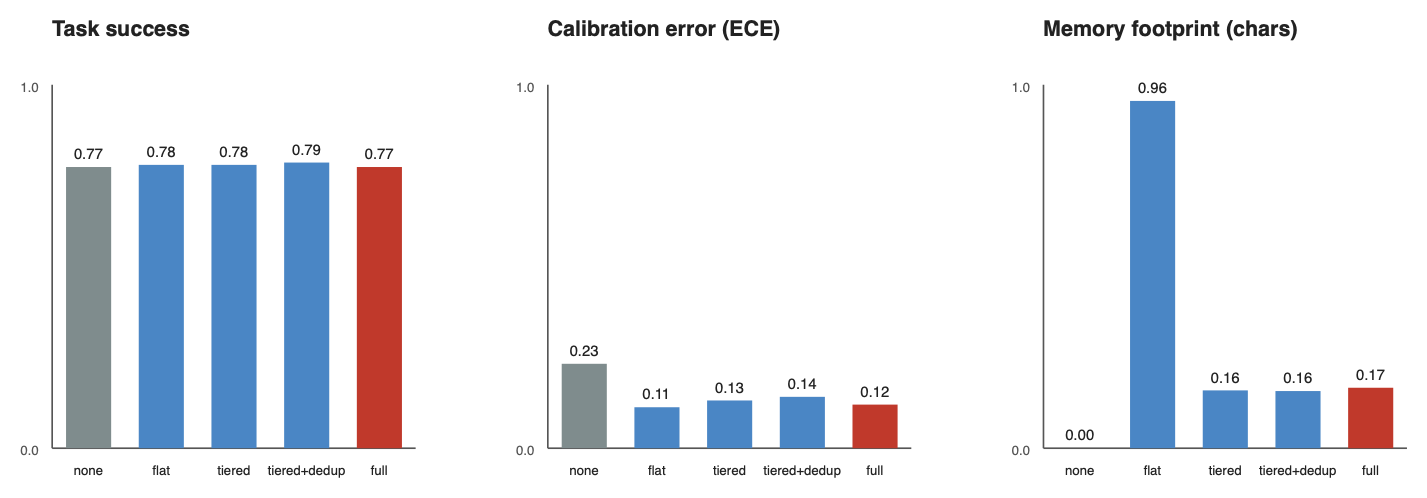
\includegraphics[width=\columnwidth]{memory.png}
\caption{Memory success, calibration, and footprint.}
\label{fig:memory}
\end{figure}

The result supports a modest claim: tiered memory is a resource-efficient calibration mechanism, not a magic source of task success. It preserves the success of flat memory while shrinking storage by an order of magnitude and keeping ECE far below the no-memory agent.

\subsection{Statistical Tests}

Isotonic selection versus embedding retrieval: success $+0.175$ (McNemar $p<0.001$), score $+0.124$ (permutation $p=0.0002$). Versus random: success $+0.325$ ($p<0.001$), score $+0.240$ ($p<0.001$). The budgeted variant versus top-1 is not tested here because it changes the action budget; it is reported as an operating point. The gate's success gain ($+0.023$) is smaller and should be read together with the negative-transfer reduction.

\section{Discussion}

\textbf{Why calibration helps.} The selector's ranking is already good before calibration (AUROC 0.842). Calibration matters because the score is consumed as a probability by the gate and by memory updates. A well-calibrated 0.4 should mean ``reuse succeeds about 40\% of the time,'' not ``the logit is above zero.'' Isotonic regression achieves this on the target distribution; temperature scaling is too rigid when the validation split is small.

\textbf{Why structural features dominate.} The benchmark's skills have explicit input requirements and spectral mechanisms. A target/input/mechanism mismatch is a hard constraint, not a subtle statistical signal. A learned model with enough data could discover this, but with 70 source tasks the hand-designed compatibility features are more sample-efficient. In real remote-sensing workflows, input requirements and target semantics are usually known and should be used.

\textbf{Why transfer diagnosis is needed.} Structural compatibility is a prior, not evidence. A land-cover classifier can look structurally incompatible with water yet work well because the water task supplies binary reference pixels. Conversely, two change detectors can look compatible yet fail on a new change type. Probe outcomes correct both errors. The Beta posterior makes the correction conservative: a skill with two positive probes is not declared transferable unless its structural prior is also reasonable, and a skill with strong evidence can override a weak prior.

\textbf{Implications for agent design.} Separate recall from commitment. Use embeddings for recall, structural checks for admissibility, calibration for probability, and a small probe budget for transfer. Keep recent episodes for adaptation and consolidated experience for scale. Do not expect memory to create skills that were never learned.

\section{Limitations and Ethics}

The benchmark is synthetic and small: $32\times32$ scenes without terrain, atmosphere, co-registration error, or real sensor noise. Skills are deterministic programs; an LLM planner would add flexibility and failure modes not captured here. The library has about 20 skills and 70 source tasks per seed, so history features are data-starved. Success thresholds are family-specific and author-specified. Eight target development tasks per family are used for transfer diagnosis; the posterior is conservative but noisy. The GeoTIFF hook is provided but not evaluated. Remote-sensing maps can inform land-use, disaster response, and environmental policy; skill reuse should be audited for mechanism mismatch and predictions should not be used without domain validation.

\section{Conclusion}

SkillEvo treats skill reuse as a calibrated decision rather than a similarity lookup. A small discriminator with structural compatibility improves top-1 success by 17.5 points over description embeddings and cuts calibration error by more than half. Tiered memory preserves success while reducing the experience footprint by 5.7$\times$. A compatibility-aware transfer diagnosis raises success by 2.3 points and reduces negative transfer. The benchmark also shows the limits of the approach: structural features dominate, history is mainly a calibration resource, and gating can only isolate non-transferable skills---not invent transferable ones.

\section*{Data and Code Availability}
The benchmark, experiment runner, task-level results, and figure-generation code are included with this manuscript under 	exttt{skillevo/} and 	exttt{experiments/}. The experiment is deterministic for a fixed seed. No proprietary data are used.

\appendices
\section{Reproducibility}

\begin{verbatim}
python -m venv .venv
source .venv/bin/activate
python -m pip install -r requirements.txt
python -m skillevo experiment --seeds 0,1,2 \
    --output experiments
python -m skillevo report
python -m unittest discover -s tests \
    -p 'test_skillevo_*.py'
\end{verbatim}

The experiment is deterministic given the seeds. The results file contains every task-level record; the generated report contains tables and figure links.

\subsection{Feature List}

Retrieval: semantic similarity, semantic rank. Compatibility: target match, family match, input match, mechanism match, band coverage, adaptivity, cost. Experience: success, utility, utility standard deviation, evidence strength, recency, coverage, duplicate rate, novelty, recent success, family-conditioned success and strength. Interactions: semantic$\times$target, input$\times$mechanism, success$\times$target.

\bibliographystyle{IEEEtran}
\bibliography{refs}

\end{document}
